% !TeX program = xelatex
% !TeX encoding = utf8
% !TeX root = slides.tex
\documentclass[xetex, onlymath, handout]{beamer}
\usefonttheme{serif}
\usetheme{hsr}

% use lmodern for math
\usepackage{lmodern}

\usepackage{tex/docmacros}

%% Pretty figures
\usepackage{circuitikz}  % Electric diagrams
\usepackage{pgfplots}    % Pretty plots
\usepackage{tikz}        % Pretty drawings
\usepackage{tikz-3dplot} % More dimensions!

\usetikzlibrary{
	external,
	calc,
	positioning,
	backgrounds,
	decorations.pathreplacing,
	calligraphy,
	decorations.markings,
	matrix,
	arrows,
	patterns,
}
\pgfplotsset{compat=newest}

% math packages
\usepackage{amsmath}
\usepackage{amssymb}

\usepackage[T1]{fontenc}
\usepackage{beramono} % monospaced
\usepackage{roboto} % other
\renewcommand*\familydefault{\sfdefault}

% metadata
\title{Multipath Fading Demonstration Platform using Software Defined Radio}
\author{Naoki Sean Pross \and Sara Cinzia Halter}
\date{Fall Semster 2021}

\institute[OST]{OST FHO Campus Rapperswil}


\begin{document}

\frame{
  \maketitle
}

\section{Multipath Fading}

\begin{frame}{Multipath fading}
	\begin{figure}
		\centering
		% vim: set ts=2 sw=2 noet:
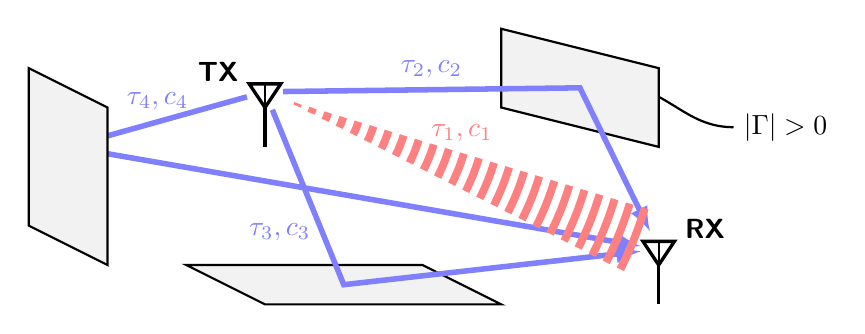
\begin{tikzpicture}[
			antenna/.pic = {
				\draw[very thick] (0,0) -- ++(2mm, 3mm) -- ++(-4mm,0) -- cycle;
				\draw[very thick] (0,0) -- ++(0,-5mm) coordinate (-mast) {};
				\draw[thick] (0,0) -- ++(0,3mm);
				\node[inner sep = 0pt, outer sep = 6pt] (-center) at (0,2mm) {};
			},
	]

	% Antennas
	\draw (0,2) pic (T) {antenna} node[above left = 3mm] {\sffamily\bfseries TX};
	\draw (5,0) pic (R) {antenna} node[above right = 3mm] {\sffamily\bfseries RX};

	% wall coefficients
	\draw[thick] (4.75, 2.25) to[out = -20, in = 180] ++(1.2,-.5) node[right] {\(|\Gamma| > 0\)};

	% walls
	\draw[thick, fill = lightgray!20] (3,2) -- ++(2,-.5) -- ++(0,1) -- ++(-2,.5) -- cycle;
	\draw[thick, fill = lightgray!20] (-1,0) -- ++(3,0) -- ++(1,-.5) -- ++(-3,0) -- cycle;


	% reflected signals
	\draw[line width = 2pt, blue!50!white, -latex] (T-center) -- node[above, pos = .5] {\(\tau_2,c_2\)} (4,2.25) -- (R-center);
	\draw[line width = 2pt, blue!50!white, -latex] (T-center) -- node[left, pos = .7] {\(\tau_3,c_3\)} (1,-.25) -- (R-center);
	\draw[line width = 2pt, blue!50!white, -latex] (T-center) -- node[above, pos = .5] {\(\tau_4,c_4\)} (-2.5,1.5) -- (R-center); 

	% another wall
	\draw[thick, fill = lightgray!20] (-2,0) -- ++(-1,.5) -- ++(0,2) --++(1,-.5) -- cycle;

	% LOS path
	\draw[line width = 1mm, red!50!white,
		decorate, decoration = {
			expanding waves, angle = 5, segment length = 2mm
		}
	] (T-center) -- node[above = 2mm, pos = .5] {\(\tau_1,c_1\)} (R-center);
\end{tikzpicture}

	\end{figure}
  \vspace{\baselineskip}
  \[
    r(t) = \sum_k c_k s(t - \tau_k).
  \]
\end{frame}



\section{Implementation}

\begin{frame}{Block Diagram}
	\begin{figure}
		\centering
		\resizebox{.9\linewidth}{!}{
			\documentclass[tikz]{standalone}

\usepackage{roboto}
\usepackage{roboto-mono}
\usepackage{tikz}        % Pretty drawings
\usepackage{tikz-3dplot} % More dimensions!
\usetikzlibrary{
	external,
	calc,
	positioning,
	backgrounds,
	decorations.pathreplacing,
	calligraphy,
	decorations.markings,
	matrix,
	arrows,
	patterns,
}
\pgfdeclarelayer{background}
\pgfdeclarelayer{foreground}
\pgfsetlayers{background,main,foreground}

\begin{document}
\documentclass[tikz]{standalone}

\usepackage{roboto}
\usepackage{roboto-mono}
\usepackage{tikz}        % Pretty drawings
\usepackage{tikz-3dplot} % More dimensions!
\usetikzlibrary{
	external,
	calc,
	positioning,
	backgrounds,
	decorations.pathreplacing,
	calligraphy,
	decorations.markings,
	matrix,
	arrows,
	patterns,
}
\pgfdeclarelayer{background}
\pgfdeclarelayer{foreground}
\pgfsetlayers{background,main,foreground}

\begin{document}
\documentclass[tikz]{standalone}

\usepackage{roboto}
\usepackage{roboto-mono}
\usepackage{tikz}        % Pretty drawings
\usepackage{tikz-3dplot} % More dimensions!
\usetikzlibrary{
	external,
	calc,
	positioning,
	backgrounds,
	decorations.pathreplacing,
	calligraphy,
	decorations.markings,
	matrix,
	arrows,
	patterns,
}
\pgfdeclarelayer{background}
\pgfdeclarelayer{foreground}
\pgfsetlayers{background,main,foreground}

\begin{document}
\include{tikz/overview.tex}
\end{document}

\end{document}

\end{document}

		}
		
	\end{figure}
\end{frame}
	
\subsection{Transmitter and Receiver Chains}

\begin{frame}{Transmitter and Receiver Chains}
	\begin{columns}
		    \begin{column}{.5\linewidth}
		    \centering
		     \includegraphics[width=\linewidth]{figures/picture/PC210002}
		    \end{column}
		    \begin{column}{.5\linewidth}
		      \begin{figure}
		      	\centering
		        \includegraphics[width=\linewidth]{figures/picture/PC210011}
		      \end{figure}
		    \end{column}
	 \end{columns}
\end{frame}


\begin{frame}{Channel model}
\begin{columns}
	\begin{column}{.5\linewidth}
		\begin{itemize}
			\item Discrete-time model
		\end{itemize}
		\vspace{0.2cm}
		\begin{figure}
			\includegraphics[width=\linewidth]{figures/screenshots/discred_time}
		\end{figure}
	\end{column}
	\begin{column}{.5\linewidth}
		\begin{itemize}
			\item Statistical model
		\end{itemize}
		\vspace{0.2cm}
		\begin{column}{.5\linewidth}
			\begin{figure}
				\includegraphics[width=\linewidth]{figures/screenshots/selectiv_1}
			\end{figure}
		\end{column}
		\begin{column}{.5\linewidth}
			\begin{figure}
				\includegraphics[width=\linewidth]{figures/screenshots/selectiv_2}
			\end{figure}
		\end{column}
	\end{column}
\end{columns}
\end{frame}





%%Tools

\end{document}

% vim:et:ts=2:sw=2:wrap:nolinebreak:
